\section{Elektrolytkondensatorens kapacitet og ESR modstandens ændring af overføringsfunktionen}\label{sec:spm4}

\begin{figure}[h!]
	\centering
	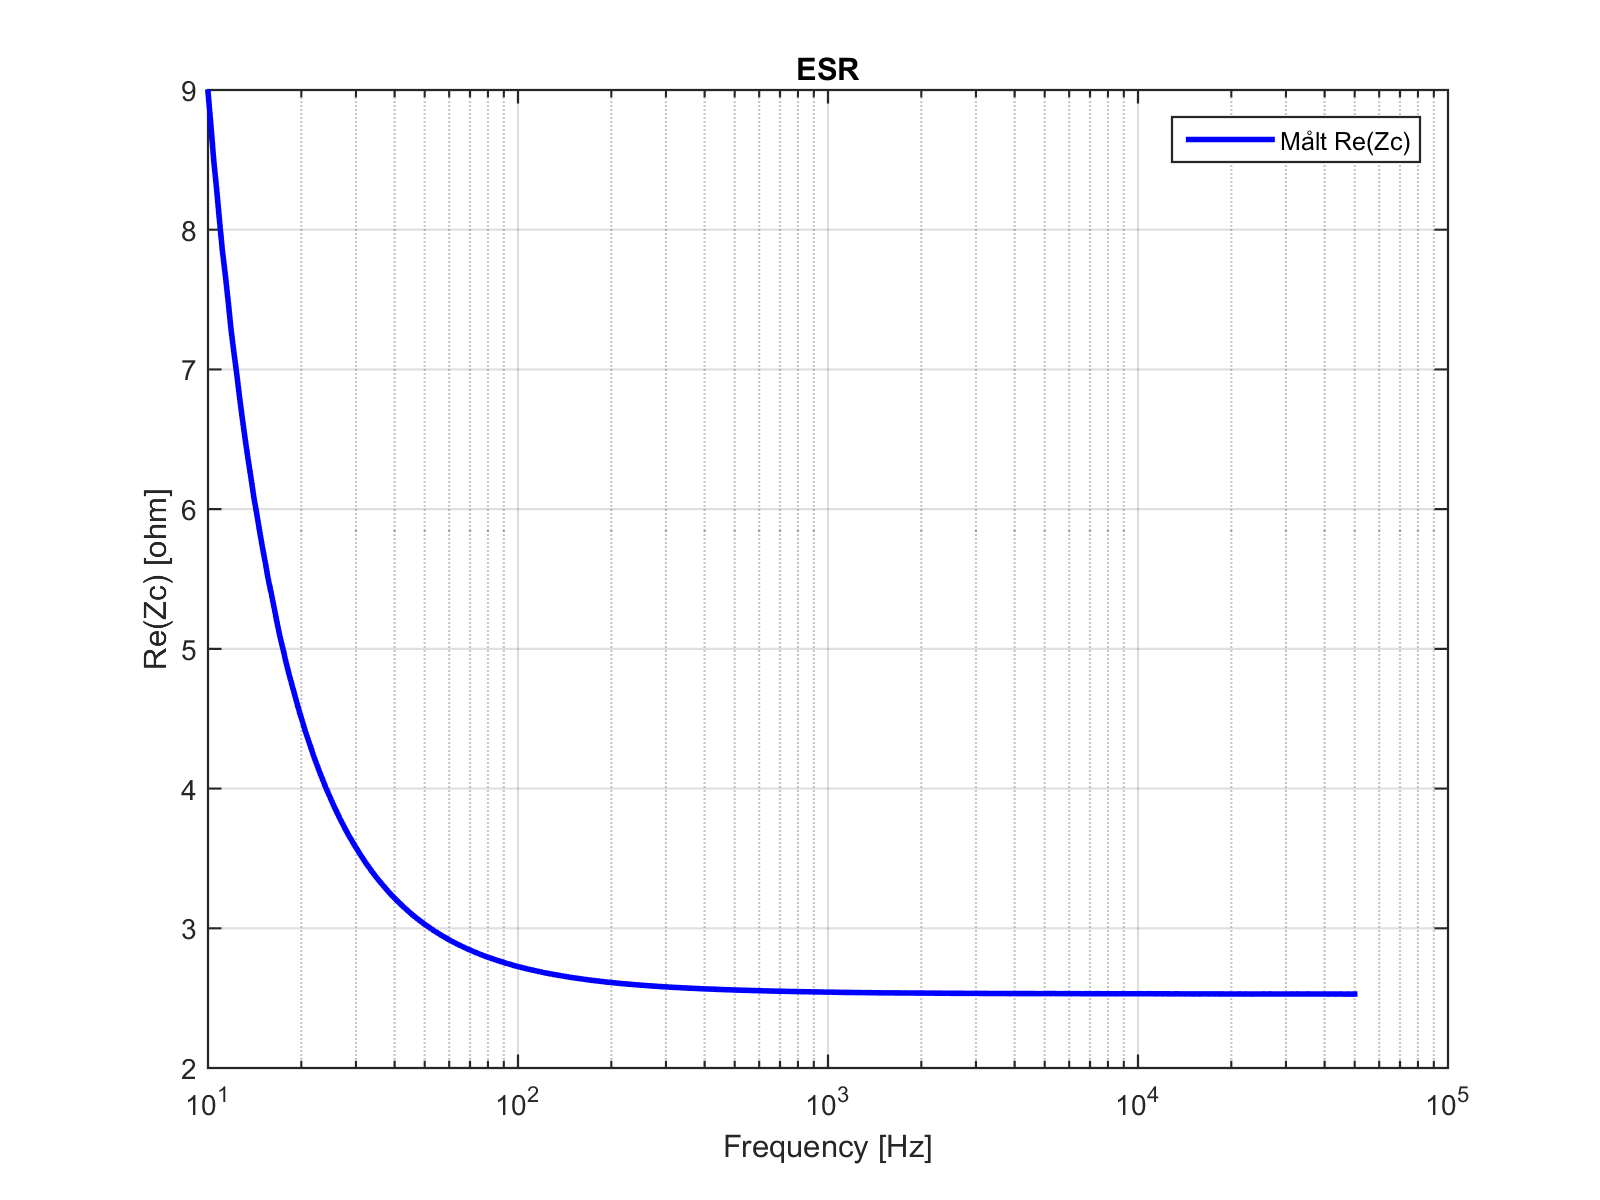
\includegraphics[width=.5\textwidth]{esrplot.png}
	\caption{Plot af ESR $Re(Zc)$, målt med Bode100.}
	\label{fig:esrplot}
\end{figure}
\FloatBlock

\begin{figure}[h!]
	\centering
	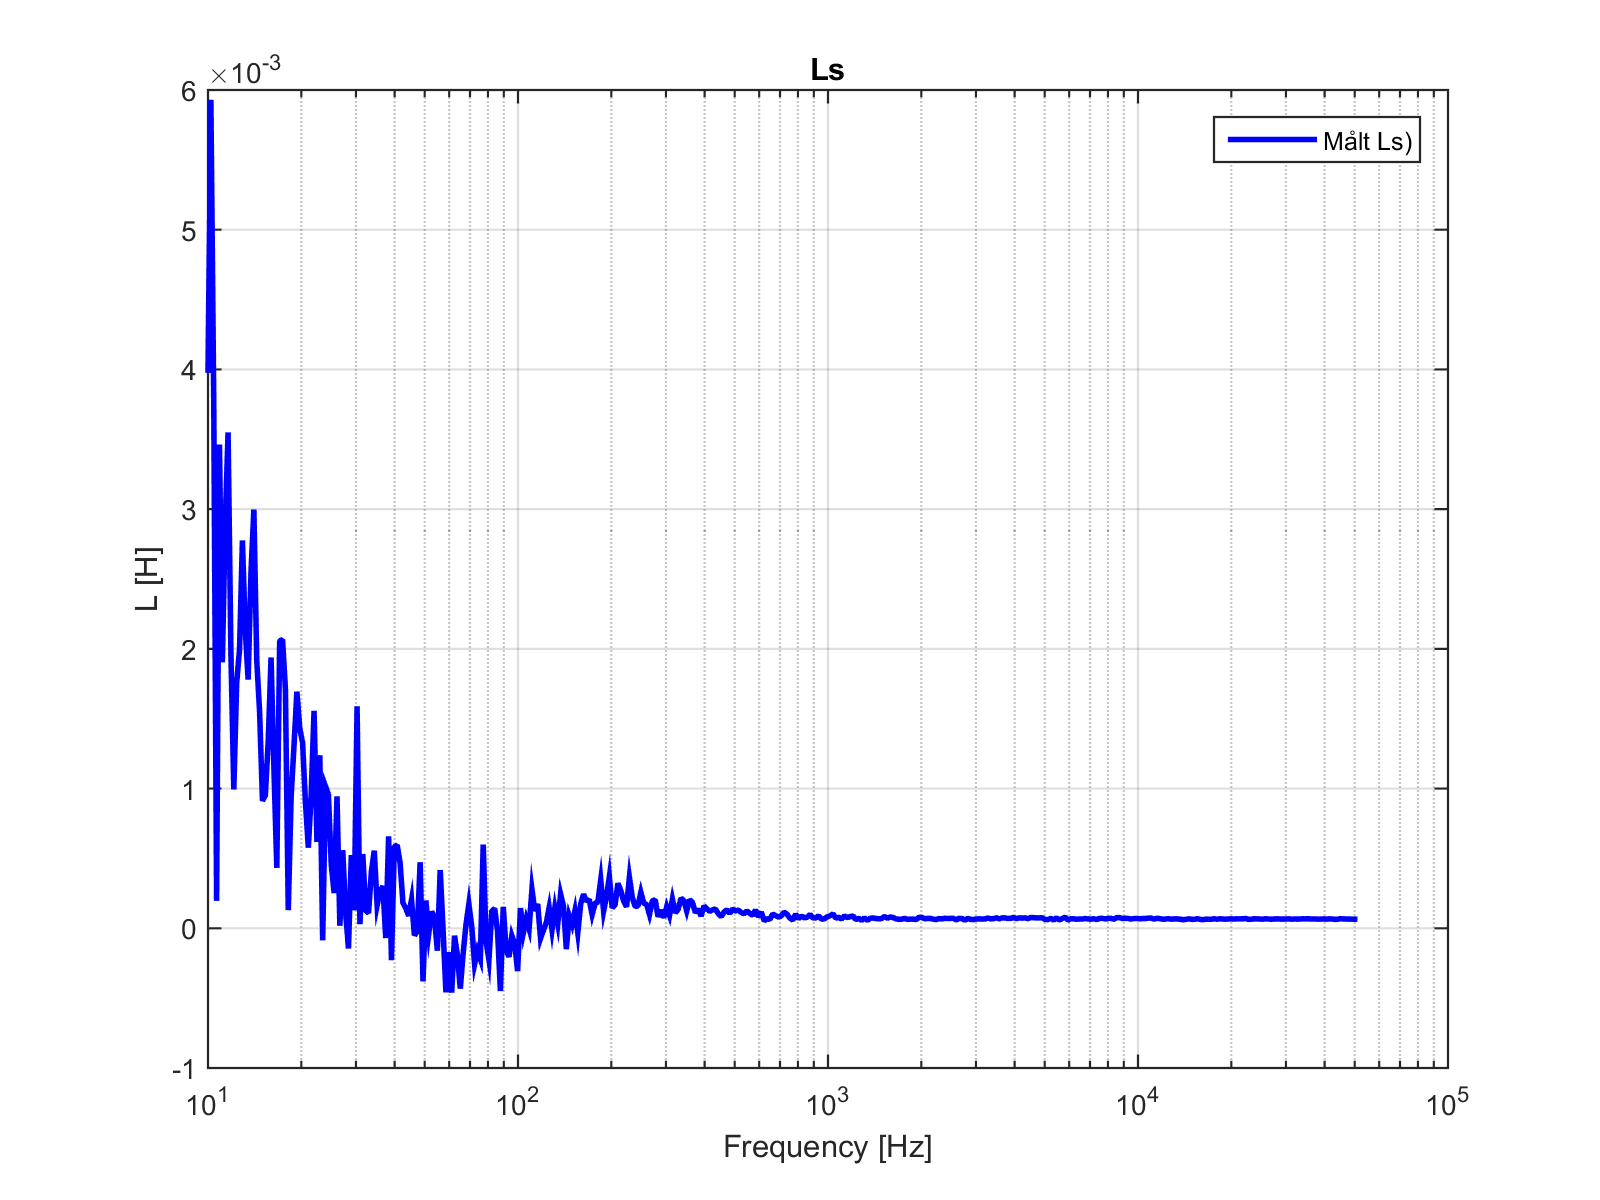
\includegraphics[width=.5\textwidth]{lsplot.png}
	\caption{Plot af Ls, målt med Bode100.}
	\label{fig:lsplot}
\end{figure}
\FloatBlock
\section*{Målinger}
Ud fra data der ligger grund for målingerne i figur \ref{fig:esrplot} og \ref{fig:lsplot} bestemmes
\begin{itemize}
	\item ESR, ved $1 \si{\kilo\hertz} \approx 2,54 \si{\ohm}$
	\item L, ved $1 \si{\kilo\hertz} \approx 82 \si{\micro\henry}$
\end{itemize} 

\section*{Noter til målinger}
Der er stor usikkerhed om de fortagede målinger er udført korrekt og derved om de fundne værdier kan bruges i efterfølgende design.
Desuden mangler måling af kondensatorens kapacitet ved resonans.